\documentclass{article}
\usepackage{etoolbox}
\usepackage{graphicx}

\ifdef{\myoutput}{}{\def\myoutput{concept}}
\ifdef{\myversion}{}{\def\myversion{1}}

\usepackage[output=\myoutput
,numberofversions=4
,version=\myversion
,seed=4
,randomizequestions=true
,randomizeanswers=true
,writeRfile=true
]{mcexam}

\usepackage[margin=0.95in]{geometry}
\usepackage{multicol}

\usepackage{fancyhdr,lastpage}
\pagestyle{fancy}
\fancyhf{}
\renewcommand{\headrulewidth}{1pt} 
\renewcommand{\footrulewidth}{1pt}
\lfoot{\mctheversion}
\rfoot{Page \thepage\ of \pageref{LastPage}}
\lhead{Quiz 8.1 and 8.3 \mctheversion \\ MAT 2000: Introduction to Statistics}
\rhead{Name Print): \hspace{2.5 in}}

\usepackage{calc}
\renewenvironment{setmcquestion}
{\begin{minipage}[t]{\linewidth-\labelwidth}}
	{\end{minipage}\par}
	
\renewenvironment{setmcquestioninstruction}
{\begin{minipage}{\textwidth}}
	{\end{minipage}}
	
\renewenvironment{setmcanswers}{}{}
\setlist[setmcquestions]{label=\mcquestionlabelfmt{*}.
	,ref=\mcquestionlabelfmt{*}
	,itemsep=0.5\baselineskip
	,topsep=1\baselineskip
}

\renewcommand\mcversionlabelfmt[1]{\arabic{#1}}

%copy-pasting from MS Word, use regex to find [\*]*[a-d]\. and replace with \answer 

\raggedbottom

\begin{document}
	Circle the correct answer for each question.  If you're unsure, you can write numbers 1, 2, 3, etc. next to the choices to get partial credit.  Questions refer to the nonindented paragraph above unless otherwise stated.\\[.5cm]
	
	\begin{mcquestions}
		\question A 1997 study described in the European Journal of Clinical Nutrition compares the growth of a random sample of vegetarian and omnivorous children, ages 7 - 11, in Northwest England. One of the aspects on which the children were compared was their body mass index (BMI). Of the 50 vegetarian children in the study, the average BMI was 16.76 and the standard deviation was 1.91. Among the 30 omnivorous children in the study, the average BMI was 17.12 and the standard deviation was 2.23.
		
		Which best describes this study design?
		\begin{mcanswerslist}
			\answer Paired using repeated measures
			\answer Paired using matching
			\answer[correct] Independent groups
			\answer None of the above
		\end{mcanswerslist}
		
		\question A random sample of medical records from 28 heart attack patients at a Boston hospital was used to better understand the relationship between cholesterol and heart failure.  The cholesterol levels of heart attack patients were recorded at 2 days and at 14 days after the patient had a heart attack.
		
		Which best describes this study design?
		\begin{mcanswerslist}
			\answer[correct] Paired using repeated measures
			\answer Paired using matching
			\answer Independent groups
			\answer None of the above
		\end{mcanswerslist}
		
		\question Researchers randomly selected 36 children who had been identified as gifted from a large city. The IQ of each child and the IQ of the child's mother were measured. A statistical analysis will be performed to determine if IQs of gifted children tend to be higher than their mothers' IQ on average.
		
		Which best describes this study design?
		
		\begin{mcanswerslist}
			\answer Paired using repeated measures
			\answer[correct] Paired using matching
			\answer Independent groups
			\answer None of the above
		\end{mcanswerslist}
		
		\begin{mcquestioninstruction}
			As part of a study, twenty students rated their own attractiveness on a scale from 1 – 10, and had a picture taken.  In the second part of the study, a group of 79 college student volunteers (not part of the original group of 20) rated the attractiveness of each of the 20 students in the pictures on a scale of 1 – 10.  Researchers averaged the attractiveness rating of the 79 "raters" (referred to as the societal rating) to compare to the self-rating to determine whether or not college students are accurate in their self-perceptions. Summary statistics are presented in the following table. The average difference in attractiveness ratings (self – societal) in the sample was 1.066 with a standard deviation of 1.507. A dotplot of these differences follows.
			\begin{center}
				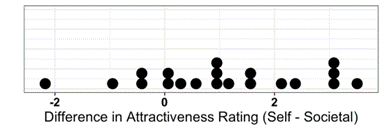
\includegraphics[width=0.8\textwidth]{self-societal.png}
			\end{center}
			Use this scenario to answer questions \ref{self-societal-1}, \ref{self-societal-2}, and \ref{self-societal-3}.
		\end{mcquestioninstruction}
		\question Would a theoretical approach be valid to analyze these data? \label{self-societal-1}
		\begin{mcanswerslist}
			\answer Yes, since the sample size of 79 is at least 20, and the distribution of differences is not strongly skewed.
			\answer Yes, since the sample size of 40 is at least 20, and the distribution of differences is not strongly skewed.
			\answer[correct] Yes, since the sample size of 20 is at least 20, and the distribution of differences is not strongly skewed.
			\answer No, a theoretical approach would not be valid because the sample size is too small.
		\end{mcanswerslist}
		
		\question[follow] Calculate the standard error of the sample mean difference in attractiveness ratings (self $–$ societal).\label{self-societal-2}
		\begin{mcanswerslist}
			\answer 1.066
			\answer 3.163
			\answer 1.507
			\answer[correct] 0.337
		\end{mcanswerslist}
		
		\question[follow] Based on the standardized statistic for this scenario, what is the conclusion? \label{self-societal-3}
		\begin{mcanswerslist}
			\answer[correct] Strong evidence exists that students similar to those in the study are not accurate in their self-perception of attractiveness, on average.
			\answer Strong evidence exists that students similar to those in the study are not accurate in their self-perception of attractiveness, on average.
			\answer No evidence exists that students similar to those in the study are not accurate in their self-perception of attractiveness, on average.
		\end{mcanswerslist}
		
		\question Researchers randomly selected 36 children who had been identified as gifted from a large city. The IQ of each child and the IQ of the child's mother were measured. A statistical analysis will be performed to determine if IQs of gifted children tend to be higher than their mothers' IQ on average. The mean difference in IQ (child – mother) was 3.22 points, with a standard deviation of 7.41 points.
		
		The p-value for these data is 0.0067. Would the results of this study be considered statistically significant at the 5\% significance level?  Select one. 
		\begin{mcanswerslist}
			\answer Yes, because random sampling was used.
			\answer No, because groups were not randomly assigned.
			\answer[correct] Yes, because the p-value is less than 0.05.
			\answer No, because the validity conditions were not met.
		\end{mcanswerslist}
		
		
	\end{mcquestions}
\end{document}